\documentclass[12pt,a4paper]{report}
\usepackage[ngerman]{babel}
\usepackage{amsmath}
\usepackage{amsfonts}
\usepackage{microtype}
\renewcommand{\baselinestretch}{1.2}
\usepackage[T1]{fontenc}
\usepackage[utf8]{inputenc}
\usepackage{lmodern}
\hyphenpenalty=10000

\usepackage{float}
\usepackage{graphicx}
\usepackage{blindtext}
\usepackage{lettrine}
\usepackage{geometry}
\usepackage{fancyhdr}
\setlength{\headheight}{15pt}
\geometry{right=3.0cm, left=4.0cm, bottom=2.5cm }

\usepackage{array}
\usepackage{titlesec}
\usepackage{color}
\usepackage{url}
\definecolor{gray75}{gray}{0.75}
\newcommand{\hsp}{\hspace{20pt}}
\titleformat{\chapter}[hang]{\Huge\bfseries}{\thechapter\hsp\textcolor{gray75}{|}\hsp}{0pt}{\Huge\bfseries}

\sloppy % Enable more relaxed line breaking
\usepackage{tikz}
\usepackage{pgfplots}

\usepackage{biblatex}
\addbibresource{quellen.bib}

\begin{document}
\begin{titlepage}
	\centering
	\includegraphics[width=0.15\textwidth]{logo.png}\par\vspace{1cm}
	{\scshape\ Bertolt-Brecht-Gymnasium \par}
	{\scshape\ Schwarzenberg \par}
	\vspace{1cm}
	{\scshape\Large Komplexe Leistung\par}
	\vspace{1.5cm}
	{\huge\bfseries Fraktale\par}
	\vspace{2cm}
	{\Large\textsc{Kevin Hoang}\par}
	\vfill
	Betreuer \par
	Herr~\textsc{Heller} \vfill
	% Bottom of the page
	{\large \today\par}
\end{titlepage}

\tableofcontents

\chapter*{Einleitung}

\addcontentsline{toc}{chapter}{\protect\numberline{}Einleitung}%

\lettrine{F}{raktale} sind faszinierende Strukturen, die uns allgegenwärtig umgeben.
Von der verzweigten Struktur eines Baumes bis hin zu den Wolken am Himmel, die sich in immer kleiner werdende Strukturen aufteilen, sind Fraktale ein fester Bestandteil unserer natürlichen Umgebung.
Aber auch in der Mathematik sind Fraktale zu finden. \newline
Der Begriff \textit{Fraktal} wurde um 1975 vom Mathematiker Benoît Mandelbrot geprägt und beschreibt natürliche und künstliche Formen, die bestimmte geometrische Eigenschaften aufweisen. \newline
Fraktale zeichnen sich durch ihre \textit{Selbstähnlichkeit} auf unterschiedlichen Größenskalen aus. Das bedeutet, dass Teile der Struktur in verschiedenen Vergrößerungen ähnliche Formen aufweisen. \newline
\hfill \break
Im theoretischen Teil dieser komplexen Leistung werde ich mich mit der mathematischen Theorie hinter Fraktalen beschäftigen, insbesondere mit der \textit{Mandelbrot-Menge} und den \textit{Julia-Mengen}. \newline
Der praktische Teil beinhaltet die Algorithmen sowie deren Implementierung zur Darstellung von Fraktalen mithilfe von Computergrafik und der Programmiersprache \textit{C++}, wobei insbesondere die \textit{OpenGL}-Bibliothek genutzt wird. \newline
\hfill \break
Ziel dieser komplexen Leistung ist es, nicht nur die mathematischen Grundlagen von Fraktalen zu verstehen, sondern auch die Ästhetik von Fraktalen zu verdeutlichen, sowie auf die Anwendung von Fraktalen in der realen Welt einzugehen.
\pagestyle{fancy}
\renewcommand{\chaptermark}[1]{\markboth{#1}{#1}}
\renewcommand{\headrulewidth}{0.4pt}

\fancyhead[L]{Fraktale}
\fancyhead[R]{\leftmark}
\chapter{Theoretischer Teil}
\thispagestyle{fancy} % Manually set the page style

In diesem Abschnitt werden die theoretischen Grundlagen erschlossen, um im
praktischen Teil ein Programm zur Darstellung von Fraktalen erstellen zu
können.

\section{Was sind Fraktale?}
Fraktale sind Strukturen, die durch die wiederholte Anwendung einfacher
Schritte aus sich selbst entstehen. Dabei weisen Fraktale auf unterschiedlichen
Größenskalen betrachtet ähnliche oder identische Formen auf, was als
Selbstähnlichkeit bezeichnet wird. Durch \textit{Iteration} werden bestimmte
Anweisungen auf immer kleiner werdenden Maßstab wiederholt, um das gewünschte
Fraktal darzustellen. \hfill \break \newline Ein anschauliches Beispiel für
diese Konzepte ist die \textit{Koch-Kurve}. Diese wird durch die iterative
Umwandlung einer geraden Linie gebildet, wobei der Mittelpunkt zu einer Spitze
umgeformt wird. Dieser Prozess wird auf den durch die Spitze neu entstandenen
Linien wiederholt, wodurch mit jeder Iteration eine immer komplexer werdende,
selbstähnliche Struktur entsteht. \newline
\begin{figure}[!htb]
  \minipage{0.30\textwidth}
  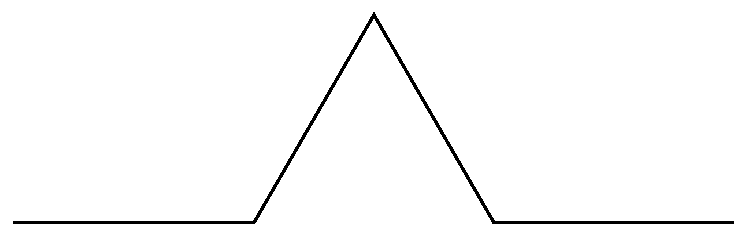
\includegraphics[width=\linewidth]{img/Koch-Kurve-1.pdf}
  \caption{\newline 1. Iteration der Koch-Kurve}\label{fig:koch_kurve_1}
  \endminipage\hfill
  \minipage{0.30\textwidth}
  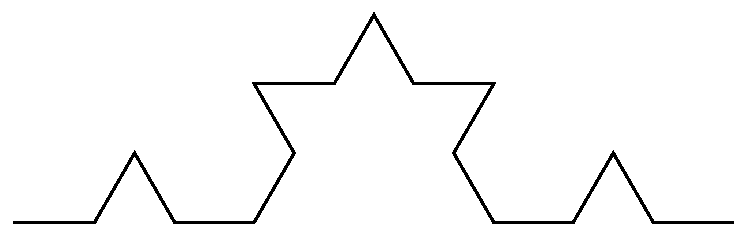
\includegraphics[width=\linewidth]{img/Koch-Kurve-2.pdf}
  \caption{\newline 2. Iteration der Koch-Kurve}\label{fig:koch_kurve_2}
  \endminipage\hfill
  \minipage{0.30\textwidth}%
  \includegraphics[width=\linewidth]{img/Koch-Kurve-3.pdf}
  \caption{\newline 3. Iteration der Koch-Kurve}\label{fig:koch_kurve_3}
  \endminipage
\end{figure}

\section{Komplexe Zahlen}

Um die Berechnung der Mandelbrot-Menge und der Julia-Mengen im nächsten
Abschnitt zu verstehen, werden zunächst die grundlegenden Konzepte zu
\textit{komplexen Zahlen} erläutert. \newline{} Komplexe Zahlen sind eine
Erweiterung der reellen Zahlen $\mathbb{R}$, mit dem Ziel, Gleichungen wie
$x^{2}=-1$ lösbar zu machen. \newline{} Eine komplexe Zahl $\mathbb{C}$ besteht
aus der Summe eines \textit{Realteils} $a$ und eines \textit{Imaginärteils} $b
  \cdot i$, wobei $b$ mit einer \textit{imaginären Einheit} $i = \sqrt{-1}$
erweitert wird und zu folgender Schreibweise führt. $$z = a + b \cdot i$$
Anders als reelle Zahlen, welche auf einem 1-dimensionalen Zahlenstrahl
dargestellt werden, verwendet man für die komplexen Zahlen die
\textit{Gauß'sche Zahlenebene}, welche einem 2-dimensionalen Koordinatensystem
gleicht. Dabei wird die $x$-Achse in den Realteil und die $y$-Achse in den
Imaginärteil eingeteilt.

% COMPLEX
\begin{figure}[h!]
  \centering
  \begin{tikzpicture}[scale=1.5]
    % Axes with ticks and labels
    \draw[->] (0,0) -- (2.5,0) node[above] {$\text{Re}$};
    \draw[->] (0,0) -- (0,2.5) node[right] {$\text{Im}$};
    % Ticks and labels on the real axis
    \foreach \x in {1,2}
    \draw (\x,0.05) -- (\x,-0.05) node[below] {$\x$};
    % Ticks and labels on the imaginary axis
    \draw (0.05,1) -- (-0.05,1) node[left] {$i$};
    \draw (0.05,2) -- (-0.05,2) node[left] {$2i$};
    % Complex number z
    \def\a{0.8}
    \def\b{1.5}
    \draw[->,thick,black] (0,0) -- (\a - 0.025,\b -0.025);
    % Points
    \filldraw[black] (\a,\b) circle (1pt) node[above right] {$z$};
    % Real and imaginary lines
    \draw[dashed] (\a,0) -- (\a,\b) -- (0,\b);
  \end{tikzpicture}
  \caption{$z=0,8 + 1,5i$ in der Gaußschen Zahlenebene}
\end{figure}
\noindent
Um mit zwei komplexen Zahlen $z=a+bi$ und $w=c+di$ rechnen zu können, gelten die folgenden Rechenregeln.
\begin{itemize}
  \item \textbf{Addition und Subtraktion}: $z \pm w = (a \pm c) + i \cdot (b \pm d)$
  \item \textbf{Multiplikation}: $z \cdot w = (ac - bd) + i \cdot (ad + bc)$
\end{itemize}
Der Betrag $\lvert z \rvert = \sqrt{a^{2}+b^{2}} $ gibt die quantitative Menge der komplexen Zahl $z$ an.

\pagebreak

\section{Mandelbrot-Menge}
Die Mandelbrot-Menge gilt als das wohl bekannteste Fraktal und wurde im Jahr
1980 vom Mathematiker Benoît Mandelbrot entdeckt. Sie beschreibt die Menge
aller komplexen Zahlen, deren Betrag bei Anwendung folgender iterativen
Vorschrift gegen einen festgelegten Grenzwert konvergiert.

$$z_{n+1} = z_{n}^{2}+ c$$

\noindent
Man beginnt mit $z_{0} = 0$ als Startwert und einer komplexen Zahl $c$ als Konstante.
Der Grenzwert, gegen den der Betrag der komplexen Zahl $z$ konvergieren soll, wird auf 2 gesetzt. Zahlen, welche diesen Grenzwert nicht überschreiten, gehören zur Mandelbrot-Menge. \newline
Zahlen, die diesen Grenzwert überschreiten, divergieren höchstwahrscheinlich ins Unendliche und gehören somit nicht zur Mandelbrot-Menge. \hfill \break \newline
\noindent
Wenn eine komplexe Zahl $c$ zur Mandelbrot-Menge gehört, zeichnet man diese
farbig in die Gauß'sche Zahlenebene ein. Diese Farbe wählt man anhand der
Anzahl der Iterationen, die benötigt werden, um den Grenzwert zu erreichen. Auf
die Farbgebung wird im praktischen Teil nochmal genauer eingegangen. \hfill \break \newline
\noindent
Die grafische Darstellung der Mandelbrot-Menge zeigt vielfältige Strukturen,
wie das charakteristische \textit{Apfelmännchen} in der Grundform mit
zahlreichen Verzweigungen am Rand. Diese Strukturen setzen sich in
selbstähnlicher Weise auf immer kleiner werdenden Maßstab fort.
% \begin{figure}[!htb]
%   \centering
%   \includegraphics[width=0.3\textwidth]{img/Mandelbrot.pdf}
%   \caption{Mandelbrot-Menge}
%   \label{fig:mandelbrot-menge}
% \end{figure}

\begin{figure}[H]
  \minipage{0.30\textwidth}
  \includegraphics[width=\linewidth]{img/Mandelbrot.pdf}
  \caption{\newline Apfelmännchen \newline}\label{fig:apfelmannchen}
  \endminipage\hfill
  \minipage{0.30\textwidth}
  \includegraphics[width=\linewidth]{img/MandelbrotZoomed.pdf}
  \caption{\newline Vergrößerung einer \newline Abzweigung}\label{fig:mandelbrot-zoomed}
  \endminipage\hfill
  \minipage{0.30\textwidth}%
  \includegraphics[width=\linewidth]{img/MandelbrotSpirals.pdf}
  \caption{\newline Spiralförmige \newline Verzweigungen}\label{fig:mandelbrot-spirals}
  \endminipage
\end{figure}

\section{Julia-Mengen}
Ein weiteres Fraktal, welches eng mit der Mandelbrot-Menge zusammenhängt, sind
die Julia-Mengen. Jeder komplexen Zahl $c$ ist eine Julia-Menge zugeordnet,
wobei die komplexen Zahlen, die auch zur Mandelbrot-Menge gehören, Julia-Mengen
erzeugen, welche ähnliche Strukturen der Mandelbrot-Menge aufweisen. \newline
Sie wurden erstmals 1918 von dem französischen Mathematiker Gaston Julia und
dem französischen Physiker Pierre Fatou beschrieben. \hfill \break \newline
Julia-Mengen werden ebenfalls durch die iterative Zahlenfolge $z_{n+1} =
  z_{n}^{2}+ c$ gebildet. Anders als bei der Mandelbrot-Menge wird jedoch der
Startwert $z_{0}$ nicht auf 0 gesetzt, sondern auf die jeweilige komplexe Zahl
$z$, für die berechnet wird, ob sie zur jeweiligen Julia-Menge der komplexen
Zahl $c$ gehört. \newline

\noindent
In der grafischen Darstellung weisen Julia-Mengen vergleichbare Eigenschaften
auf wie die Mandelbrot-Menge. Ihre Strukturen sind jedoch weniger komplex,
gleichen aber den jeweiligen Strukturen der Mandelbrot-Menge.

\hfill \break
\newline

\begin{figure}[!htb]
  \minipage{0.30\textwidth}
  \includegraphics[width=\linewidth]{img/Julia -1.0+0.4i.pdf}
  \caption{\newline Julia-Menge für \newline $c=-1.0+4.0i$}\label{fig:julia-menge-1}
  \endminipage\hfill
  \minipage{0.30\textwidth}
  \includegraphics[width=\linewidth]{img/Julia -0.8+0.2i.pdf}
  \caption{\newline Julia-Menge für \newline  $c = -0,8 + 0,2i$}\label{fig:julia-menge-2}
  \endminipage\hfill
  \minipage{0.30\textwidth}%
  \includegraphics[width=\linewidth]{img/Julia -0.8+0.0i.pdf}
  \caption{\newline Julia-Menge für \newline  $c = -0,8 + 0,0i$}\label{fig:julia-menge-3}
  \endminipage
\end{figure}
\chapter{Praktischer Teil}
\thispagestyle{fancy} % Manually set the page style

\section{C++ und OpenGL}
\blindtext 


\section{Programmaufbau}
\blindtext 


\section{Implementierung der Algorithmen}
\blindtext 


% \section{Limitationen} %
\chapter{Fazit}
\thispagestyle{fancy} % Manually set the page style

\section{Zusammenfassung der Ergebnisse}
\blindtext 


\section{Anwendungsmöglichkeiten von Fraktalen}
\blindtext 

\titlespacing*{\chapter}{0pt}{-30pt}{20pt}

\chapter{Anhang}
\thispagestyle{fancy} % Manually set the page style

\section{Quellcode}
Der Quellcode und das Programm sind über den beigelegten USB-Stick oder über
folgenden GitHub Link verfügbar: \newline
\url{https://www.github.com/kevinoverflow/Fraktale}
% \section{Abbildungen} %
\section{Bibliotheken}
\subsubsection*{CMake - \url{https://cmake.org/}}
\textit{Ein plattformübergreifendes Open-Source-Build-System.}
\subsubsection*{CMakeRC - \url{https://github.com/vector-of-bool/cmrc}}
\textit{Ein Ressourcencompiler in einem einzigen CMake-Skript.}
\subsubsection*{Dear ImGui - \url{https://github.com/ocornut/imgui}}
\textit{Eine einfache Immediate-Mode-Grafikbenutzeroberfläche für C++.}
\subsubsection*{GLFW - \url{https://www.glfw.org/}}
\textit{Eine plattformübergreifende Bibliothek zur Erstellung von Fenstern mit OpenGL-Kontexten.}
\subsubsection*{GLEW - \url{http://glew.sourceforge.net/}}
\textit{Die OpenGL Extension Wrangler Library für eine einfachere Handhabung von OpenGL-Erweiterungen.}
\subsubsection*{GLM - \url{https://glm.g-truc.net/0.9.9/index.html}}
\textit{OpenGL Mathematics (GLM) ist eine rein Header basierte C++-Mathematikbibliothek für Grafiksoftware, basierend auf den Spezifikationen der OpenGL Shading Language (GLSL).}
\newpage
\section{Literaturverzeichnis}
\printbibliography[heading=none]
\chapter*{Selbstständigkeitserklärung}

Ich versichere, dass ich die Komplexe Leistung ohne fremde Hilfe angefertigt, andere als die angegebenen Quellen und Hilfsmittel nicht benutzt und mich auch sonst keiner unerlaubten Hilfe bedient habe. Alle wörtlich oder sinngemäß übernommenen Textstellen habe ich als solche kenntlich gemacht.
\\[2ex]
Schwarzenberg, den 21. Dezember 2023
\flushleft
\newlength\us
\settowidth{\us}{-Kevin Hoang-}
\vspace{1cm}
\begin{tabular}{p{\us}}\hline
\centering\footnotesize Kevin Hoang
\end{tabular}


\end{document}